\documentclass{article}\usepackage[]{graphicx}\usepackage[]{color}
%% maxwidth is the original width if it is less than linewidth
%% otherwise use linewidth (to make sure the graphics do not exceed the margin)
\makeatletter
\def\maxwidth{ %
  \ifdim\Gin@nat@width>\linewidth
    \linewidth
  \else
    \Gin@nat@width
  \fi
}
\makeatother

\definecolor{fgcolor}{rgb}{0.345, 0.345, 0.345}
\newcommand{\hlnum}[1]{\textcolor[rgb]{0.686,0.059,0.569}{#1}}%
\newcommand{\hlstr}[1]{\textcolor[rgb]{0.192,0.494,0.8}{#1}}%
\newcommand{\hlcom}[1]{\textcolor[rgb]{0.678,0.584,0.686}{\textit{#1}}}%
\newcommand{\hlopt}[1]{\textcolor[rgb]{0,0,0}{#1}}%
\newcommand{\hlstd}[1]{\textcolor[rgb]{0.345,0.345,0.345}{#1}}%
\newcommand{\hlkwa}[1]{\textcolor[rgb]{0.161,0.373,0.58}{\textbf{#1}}}%
\newcommand{\hlkwb}[1]{\textcolor[rgb]{0.69,0.353,0.396}{#1}}%
\newcommand{\hlkwc}[1]{\textcolor[rgb]{0.333,0.667,0.333}{#1}}%
\newcommand{\hlkwd}[1]{\textcolor[rgb]{0.737,0.353,0.396}{\textbf{#1}}}%
\let\hlipl\hlkwb

\usepackage{framed}
\makeatletter
\newenvironment{kframe}{%
 \def\at@end@of@kframe{}%
 \ifinner\ifhmode%
  \def\at@end@of@kframe{\end{minipage}}%
  \begin{minipage}{\columnwidth}%
 \fi\fi%
 \def\FrameCommand##1{\hskip\@totalleftmargin \hskip-\fboxsep
 \colorbox{shadecolor}{##1}\hskip-\fboxsep
     % There is no \\@totalrightmargin, so:
     \hskip-\linewidth \hskip-\@totalleftmargin \hskip\columnwidth}%
 \MakeFramed {\advance\hsize-\width
   \@totalleftmargin\z@ \linewidth\hsize
   \@setminipage}}%
 {\par\unskip\endMakeFramed%
 \at@end@of@kframe}
\makeatother

\definecolor{shadecolor}{rgb}{.97, .97, .97}
\definecolor{messagecolor}{rgb}{0, 0, 0}
\definecolor{warningcolor}{rgb}{1, 0, 1}
\definecolor{errorcolor}{rgb}{1, 0, 0}
\newenvironment{knitrout}{}{} % an empty environment to be redefined in TeX

\usepackage{alltt}[12pt]
\usepackage{Sweave}
\usepackage{float}
\usepackage{graphicx}
\usepackage{tabularx}
\usepackage{siunitx}
\usepackage[margin=2.5cm]{geometry}
\usepackage{pdflscape}
\usepackage{mdframed}
\usepackage{natbib}
\bibliographystyle{..//refs/styles/besjournals.bst}
\usepackage[small]{caption}
\setlength{\captionmargin}{30pt}
\setlength{\abovecaptionskip}{0pt}
\setlength{\belowcaptionskip}{10pt}
%\topmargin -2.5cm        
%\oddsidemargin -2.5cm   
%\evensidemargin -2.5cm
\textwidth 16.59cm
\textheight 21.94cm 
%\pagestyle{empty} %comment if want page numbers
\parskip 7.2pt
\renewcommand{\baselinestretch}{2}
\parindent 0pt
\usepackage{lineno}
\linenumbers
\usepackage{setspace}
\doublespacing

\newmdenv[
  topline=true,
  bottomline=true,
  skipabove=\topsep,
  skipbelow=\topsep
]{siderules}

%% R Script


\IfFileExists{upquote.sty}{\usepackage{upquote}}{}
\begin{document}
\noindent \textbf{\Large{Rethinking False Spring Risk}}

\noindent Authors:\\
C. J. Chamberlain $^{1,2}$, B. I. Cook $^{3}$, I. Garcia de Cortazar Atauri $^{4}$ \& E. M. Wolkovich $^{1,2,5}$
\vspace{2ex}\\
\emph{Author affiliations:}\\
$^{1}$Arnold Arboretum of Harvard University, 1300 Centre Street, Boston, Massachusetts, USA; \\
$^{2}$Organismic \& Evolutionary Biology, Harvard University, 26 Oxford Street, Cambridge, Massachusetts, USA; \\
$^{3}$NASA Goddard Institute for Space Studies, New York, New York, USA; \\
$^{4}$French National Institute for Agricultural Research, INRA, US1116 AgroClim, F-84914 Avignon, France\\
$^{5}$Forest \& Conservation Sciences, Faculty of Forestry, University of British Columbia, 2424 Main Mall, Vancouver, BC V6T 1Z4\\
\vspace{2ex}
$^*$Corresponding author: 248.953.0189; cchamberlain@g.harvard.edu\\

\noindent \emph{Keywords:} false spring, phenology, freezing tolerance, climate change, forest communities \\
%\tableofcontents
\emph{Paper type:} Opinion
%\emph{Counts}: Total word count for the main body of the text:  2611; Abstract: 119; 4 figures (all in color). \\

\renewcommand{\thetable}{\arabic{table}}
\renewcommand{\thefigure}{\arabic{figure}}
\renewcommand{\labelitemi}{$-$}
\setkeys{Gin}{width=0.8\textwidth}

%%%%%%%%%%%%%%%%%%%%%%%%%%%%%%%%%%%%%%%%%%%%%%%
% General to do
% Move all figures and their captions to end of manuscript
% Work on transitions throughout. I made note of it many places.
% My comments are usually in [] and I made some edits throughout. You can use the app FileMerge (spotlight search for it) on most Macs to see the changes quickly. 
%%%%%%%%%%%%%%%%%%%%%%%%%%%%%%%%%%%%%%%%%%%%%%%

\newpage
\section*{Abstract}
Temperate plants are at risk of being exposed to late spring freezes --- often called false springs --- which can be damaging ecologically and economically. As climate change may alter the prevalence and severity of false springs, our ability to accurately forecast such events has become more critical. Currently, many false spring studies simplify the ecological and physiological information needed for accurate predictions of the level of plant damage from late spring freezes. Here we review the complexity of factors driving a plant's false spring risk. We highlight how species, life stage, and habitat differences contribute to the damage potential of false springs. %(The ultimate intent is to demonstrate how an integrated view of false spring that incorporates these factors would rapidly advance progress in this field.)
Integrating these complexities could rapidly advance forecasting of false spring events in climate change and ecological studies.
% In this paper we aim to highlight the complexity of factors driving a plant's false spring risk and provide a road map for improved metrics. First, we review the currently used definitions of false spring. Then, combining research from plant physiology, climatology and community ecology, we outline major gaps in current definitions.

\section*{Introduction}

Plants from temperate environments time their growth each spring to follow rising temperatures alongside increasing light and soil resource availability. While tracking spring resource availability, individuals that budburst before the last freeze date are at risk of leaf loss, damaged wood tissue, and slowed canopy development \citep{Gu2008, Hufkens2012}. These damaging late spring freezes are also known as false springs, and are widely documented to result in adverse ecological and economic consequences \citep{Ault2013, Knudson2012}.

Climate change is expected to cause an increase in damage from false spring events due to earlier spring onset and potentially greater fluctuations in temperature in some regions \citep{Inouye2008, Martin2010}. Already, multiple studies have documented false springs in recent years \citep{Augspurger2009, Augspurger2013, Gu2008, Menzel2015} and some have linked these events to climate change \citep{Allstadt2015, Ault2013,  Muffler2016, Vitra2017, Xin2016}. This interest in false springs has led to a growing body of research investigating the effects on temperate forests. For this research to produce accurate predictions, however, researchers need methods that properly evaluate the effects of false springs across diverse species and climate regimes. 

\subsection*{Measuring False Spring}
Current metrics for estimating false springs events are generally simple, often requiring an estimate for the start of biological `spring' (i.e. budburst) and whether temperatures below a particular threshold occurred in the following week. Such estimates inherently assume consistency of damage across species, functional group, life stages, and other climatic regimes, ignoring that such factors can greatly impact plants' false spring risk. As a result, such indices may lead to inaccurate estimates and predictions. % CUTFORLENGTH: slowing our progress in understanding false spring events and how they may shift with climate change. 

In this paper we highlight the complexity of factors driving a plant's false spring risk and provide a road map for improved metrics. We show how location within a forest or canopy \citep{Augspurger2013}, interspecific variation in avoidance and tolerance strategies \citep{Martin2010, Muffler2016}, freeze temperature thresholds \citep{Lenz2013}, and regional effects \citep{Muffler2016} unhinge simple metrics of false spring. We argue that a new approach that integrates these and other crucial factors would help accurately determine current false spring damage and improve predictions of spring freeze risk under a changing climate --- while potentially providing novel insights to how plants respond to and are shaped by spring frost. % The ultimate intent is to demonstrate how an integrated view of false spring that incorporates these factors would rapidly advance progress in this field.  

\section*{Defining False Spring: An example in one temperate plant community}
Temperate forest plants experience elevated risk of frost damage during the spring due to the stochastic timing of frosts. Freezing temperatures following a warm spell can result in plant damage or even death \citep{Ludlum1968, Mock2007}. Many temperate species exhibit flexible spring phenologies, which help them minimize spring freezing risk, but freeze damage can still occur. Once buds exit the dormancy phase, they are less freeze tolerant and less resistant to ice formation \citep{ Lenz2013, Taschler2004, Vitasse2014a}. Intracellular ice formation from false spring events often results in severe leaf and stem damage \citep{Burke1976, Sakai1987}. Ice formation can also occur indirectly (i.e. extracellularly), which results in freezing dehydration and mimics drought conditions \citep{Beck2004, Hofmann2015, Pearce2001}. Both forms of ice formation can cause defoliation and crown dieback \citep{Gu2008}. 
An effective and consistent definition of false spring would accurately determine the amount and type of ice formation to properly evaluate the level of damage that could occur.
 

Currently there are several ways to define a false spring. A common definition describes a false spring as having two phases: rapid vegetative growth prior to a freeze and a post freeze setback \citep{Gu2008}. Other definitions instill more precise temporal parameters, specific to certain regions \citep[e.g., in][false spring for the Midwestern United States is defined as a warmer than average March, a freezing April, and enough growing degree days between budburst and the last freeze date]{Augspurger2013}. A widely used definition integrates a mathematical equation to quantify a false spring event. This equation, known as a False Spring Index (FSI), signifies the likelihood of damage to occur from a late spring freeze. Currently, FSI is evaluated annually by the day of budburst and the day of last spring freeze \citep[often calculated at -2.2$^{\circ}$C,][]{Schwartz1993} through the simple equation \citep{Marino2011}:
\begin{equation} \label{eq:1}
FSI = \text{Day of Year} (Last Spring Freeze) - \text{Day of Year} (Budburst)
\end{equation}
Negative values indicate no risk situations, whereas a damaging FSI is currently defined to be 7 or more days between budburst and the last freeze date (Equation \ref{eq:1}) \citep{Peterson2014}. This 7 day threshold captures the reality that leaf tissue is at high risk of damage from frost in the period after budburst, with later vegetative phases (e.g., after full leafout) being more resistant to such damage.% OLD: By using the 7 day threshold, it is likely less resistant vegetative phenophases will be exposed to a false spring, thus putting the plant at a higher risk of damage. 

To demonstrate how the FSI definition works, we applied it to data from the Harvard Forest Long-term Ecological Research program in Massachusetts. We used three separate methodologies to calculate spring onset: long-term ground observational data \citep{Okeefe2014}, PhenoCam data from Harvard Forest \citep{Richardson2015}, and USA National Phenology Network's (USA-NPN) Extended Spring Index (SI-x) data \citep{USA-NPN2016}. These spring onset values were then inputted into the FSI equation (Equation \ref{eq:1}) to calculate FSI from 2008 to 2014 (Figure \ref{fig:fsifig}). 

Each methodology rendered different FSI values, suggesting different false spring damage for the same site and same year. For most years, the observational FSI and PhenoCam FSI are about 10-15 days lower than the SI-x data. This is especially important for 2008, when the SI-x data indicates a false spring year, whereas the other two datasets do not. In 2012, the observational data and PhenoCam data diverge slightly and the PhenoCam FSI is over 30 days less than the SI-x value.

The reason for these discrepancies is that each method evaluates spring onset by integrating different attributes such as age, species or functional group. Spring phenology in temperate forests typically progresses by functional group: understory species and young trees tend to initiate budburst first, whereas larger canopy species start later in the season \citep{Richardson2009, Xin2016}. The different FSI values determined in Figure \ref{fig:fsifig} exemplify the differences in functional group spring onset dates and illustrate variations in forest demography and phenology. While the SI-x data (based on observations of early-active shrub species, including lilac, \emph{Syringa vulgaris}) may best capture understory dynamics, the PhenoCam and observational FSI data integrate over larger canopy species. Such differences are visible each year, as the canopy-related metrics show lower risk, but are especially apparent in 2012. In 2012, a false spring event was reported through many regions of the US due to warm temperatures occurring in March \citep{Ault2015}. These high temperatures would most likely have been too early for larger canopy species to initiate budburst but they would have affected smaller understory species, as is seen by the high risk of the SI-x FSI in Figure \ref{fig:fsifig}. 

Yet, in contrast to our three metrics of spring onset for one site, most FSI work currently ignores variation across functional groups --- instead using one metric of spring onset and assuming it applies to the whole community of plants \citep{Allstadt2015, Marino2011, Mehdipoor2017, Peterson2014}. The risk of a false spring varies across habitats and with species composition since spring onset is not consistent across functional groups \citep{Martin2010}. Therefore, one spring onset date cannot be used as an effective proxy for all species. False spring studies should first assess the forest demographics and functional groups relevant to the study question in order to effectively estimate the date of spring onset. However, as we outline below, considering different functional groups is unlikely to be enough for robust predictions. It is also important to integrate species differences within functional groups and to consider the various interspecific avoidance and tolerance strategies that species have evolved against false springs. 

\section* {Plant Physiology and Diversity versus the Current False Spring Definition}
Plants have evolved to minimize false spring damage through two strategies: avoidance and tolerance. Many temperate forest plants utilize various morphological strategies to be more frost tolerant: some have increased `packability' of leaf primordia in winter buds, which may permit more rapid leafout \citep{Edwards2017} and minimize the exposure time of less resistant tissues. Other species have young leaves with more trichomes to act as a buffer against spring frosts \citep{Agrawal2004, Prozherina2003}. And many other individuals are able to respond to abiotic cues such as consistently dry winters. Species living in habitats with drier winters develop shoots and buds with decreased water content, which makes the buds more tolerant to drought and also to false spring events \citep{Beck2007, Kathke2011, Hofmann2015, Morin2007,  Muffler2016, Nielsen2009, Poirier2010}. These strategies are probably only a few of the many ways plants work to morphologically avoid frost damage, and more studies are needed to investigate the interplay between morphological traits and false spring tolerance. 

Rather than being more tolerant of spring freezing temperatures, some temperate forest species have evolved to avoid frosts via their phenologies. Effective avoidance strategies require well-timed spring phenologies. Most temperate deciduous tree species optimize growth and minimize spring freeze damage by using three cues to initiate budburst: low winter temperatures (chilling), warm spring temperatures (forcing), and increasing photoperiods \citep{Chuine2010}. The evolution of these three cues and their interactions has permitted temperate plant species to occupy more northern ecological niches \citep{Kollas2014} and decrease the risk of false spring damage %, which is crucial for avoidance strategies 
\citep{Charrier2011}. One avoidance strategy, for example, is the interaction between over-winter chilling and spring forcing temperatures. Warm temperatures earlier in the winter %(i.e. in February, or even January in the Mediterranean) %% CJC: removed due to failure to acknowledge Southern Hemisphere
will not result in early budburst due to insufficient chilling \citep{Basler2012}. Likewise, photoperiod sensitivity is a common false spring avoidance strategy: species that respond strongly to photoperiod cues in addition to warm spring temperatures are unlikely to have large advances in budburst with warming, and thus may evade false spring events as warming continues \citep{Basler2014}. 
% Given the diverse array of spring freezing defense mechanisms, predicting damage by false spring events requires a greater understanding of avoidance and tolerance strategies across species, especially with a changing climate.

\section* {Defining Vegetative Risk} % Complexities due to Species' Strategies and Climate
%% CJC (3-Jul-2018) made tweaks to paragraph below
Phenology and frost tolerance are intertwined --- with important variation occurring across different phenological phases. Flowering and fruiting are generally more sensitive to false spring events than vegetative phases \citep{Augspurger2009, Caradonna2016, Lenz2013}, but false spring events that occur during the vegetative growth phenophases may impose the greatest freezing threat to deciduous plant species.  Plants will suffer greater long-term effects from the loss of photosynthetic tissue, which could impact multiple years of growth, reproduction, and canopy development \citep{Vitasse2014, Xie2015}. However, there is high variability in defining a damaging temperature threshold across species, including between agricultural and ecological studies (Figure \ref{fig:temp}).

There is also important variation within certain phenological phases. Most notably, within the vegetative phases of spring leafout, plants that have initiated budburst but have not fully leafed out are more likely to sustain damage from a false spring than individuals past the leafout phase. This is because freezing tolerance is lowest after budburst begins until the leaf is fully unfolded \citep{Lenz2016}. Therefore, the rate of budburst and the length of time between budburst and leafout is essential for predicting the level of damage from a false spring event. We will refer to the timing between these phenophases --- budburst to leafout --- as the duration of vegetative risk (Figure \ref{fig:risk}). % CUT FOR LENGTH: The duration of vegetative risk can be extended if a freezing event occurs during the phenophases between budburst and full leafout \citep{Augspurger2009}, which could result in exposure to multiple frost events in one season.

\section* {How Species Phenological Cues Shape Vegetative Risk}
Predictions of false spring critically depend on understanding what controls the duration of vegetative risk across species. For temperate species, the three major cues (winter chilling temperatures, spring warming temperatures and photoperiod) that control budburst \citep%[e.g., low winter temperatures, warm spring temperatures, and increasing photoperiods]
{Chuine2010} play a dominant role. Most phenological studies currently focus on one phenophase (i.e. budburst or leafout) but, to examine false spring risk, it is important to examine the effects of the three phenological cues and their interactions on the duration of vegetative risk---that is, researchers must collect data on both budburst and leafout timing.  

Such cues may provide a starting point for predicting how climate change will alter the duration of vegetative risk. Robust predictions will require more information, especially the emissions scenario realized over coming decades \citep{IPCC2014}, but some outcomes with warming are more expected than others. For example, higher temperatures are generally expected to increase forcing and decrease chilling in many locations, as well as to trigger budburst at times of the year when daylength is shorter. Using data from a recent study that manipulated all three cues and measured budburst and leafout \citep{Flynn2018} shows that any one of these effects alone can have a large impact on the duration of vegetative risk (Figure \ref{fig:dan}): more forcing shortens it substantially (-15 to -8 days), while shorter photoperiods and less chilling increase it to a lesser extent (+3 to 9 days). Together, however, the expected shifts generally shorten the duration of vegetative risk by 4-13 days, both due to the large effect of forcing and the combined effects of multiple cues. How shortened the risk period is, however, varies strongly by species and highlights how climate change may speed some species through this high risk period, but not others. Additionally, as our results are for a small set of species we expect other species may have more diverse responses, as has already been seen in shifts in phenology with warming \citep{Cleland2006, Fu2015, Xin2016}.

These findings highlight the need for further studies on the interplay between chilling, forcing, and photoperiod cues and the duration of vegetative risk across species. This is especially true for species occupying ecological niches more susceptible to false spring events; even if warming causes a shortened duration of vegetative risk for such species, the related earlier budburst dates could still lead to greater risk of false spring exposure.

% show that predictions will require accurate forecasts of the magnitude and direction of how forcing, daylength and chilling will change in the future, as well as how those cues vary across species. 
%Considering the interaction of cues and climate change further complicates understanding species future vulnerabilities to false spring events.  %For example, as climate change progresses, higher spring forcing temperatures may be required for species experiencing insufficient winter chilling (due to warmer winter temperatures), especially at lower latitudes \citep{McCreary1990, Morin2009, Fu2012, Polgar2014, Chuine2010}. 
% Individuals that initiate budburst earlier in the spring may attempt to limit freezing risk by decreasing the duration of vegetative risk in order Further studies are essential 

\subsection* {Predictable Regional Differences in Climate, Species Responses and False Spring Risk}
Robust predictions must consider the interplay of species cues with a specific location's climate. Climate and thus false spring risk vary across regions. Some regions experience harsher winters and greater temperature variability throughout the year (Figure \ref{fig:region} e.g. Maine, USA), and these more variable regions often have a much higher risk of false spring than others (Figure \ref{fig:region} e.g. Lyon, France). Understanding and integrating such spatiotemporal effects and regional differences when investigating false spring risk and duration of vegetative risk would help improve predictions as climate change progresses. Such differences depend both on the local climate, the local species and the cues for each species at that location, as a single species may have varying cues across space. Therefore, based on cues alone, different regions may have different durations of vegetative risk for the same species \citep {Caffarra2011, Partanen2004, Viheraaarnio2006}. Studies also show that different species within the same location can exhibit different sensitivities to the three cues \citep{Basler2012, Laube2013}, further amplifying the myriad of climatic and phenological shifts that determine false spring risk in a region. 
% CJC (3-Jul-2018): various studies that investigated latitudinal effects indicate that populations growing further north respond to a different interaction of cues than those growing further south. Thus, 

How a single species phenological cues varies across space is not yet well predicted. Some studies have investigated how phenological cues for budburst vary across space, including variation across populations, by using latitudinal gradients \citep{Gauzere2017, Sogaard2008, Way2015, Zohner2016}. Fewer, however, have integrated distance from the coast \citep [but see][]{Aitken2015, Harrington2015, Myking2007} or regional effects. Some studies assert that the distance from the coast is a stronger indicator of budburst timing than latitude \citep{Myking2007}, with populations further inland initiating budburst first, whereas those closer to the coast budburst later in the season. Therefore, to better understand the interplay between duration of vegetative risk and climatic variation it is important to recognize how climate regime extremes (e.g. seasonal trends, annual minima and annual maxima) vary across regions and how they will shift in the future: as climatic regimes are altered by climate change false spring risk could vary in intensity across regions and time (i.e. regions currently at high-risk of false spring damage could become low-risk regions in the future and vice versa). 

%Accurate predictions need to carefully consider how chilling and forcing cues vary across regions. [WHAT ABOUT PHOTOPERIOD? How is this paragraph different from the above? Should we combine them?]
%Climatic variation across regions and at different distances from the coast results in varying durations of vegetative risk due to different chilling and forcing temperatures . 

\section*{Conclusion}
Temperate forest trees are most at risk to frost damage in the spring due to the stochasticity of spring freezes. With warm temperatures advancing in the spring but last spring freeze dates advancing at a slower rate, there could be more damaging false spring events in the future, especially in high-risk regions \citep{Gu2008, Inouye2008, Liu2018}. Current equations for evaluating false spring damage (e.g. Equation \ref{eq:1}) largely simplify the myriad complexities involved in assessing false spring damage and risks. More studies aimed at understanding relationships between species avoidance and tolerance strategies, climatic regimes, and physiological cue interactions with the duration of vegetative risk would improve predictions. Additionally, research to establish temperature thresholds for damage across functional types and phenophases will help effectively predict false spring risk in the future. An integrated approach to assessing past and future spring freeze damage would provide novel insights into plant strategies, and offer more robust predictions as climate change progresses, which is essential for mitigating the adverse ecological and economic effects of false springs.

\section*{Acknowledgments}
We thank D. Buonaiuto,  W. Daly, A. Ettinger, and I. Morales-Castilla for comments and insights that improved the manuscript. 

\nocite{Soudani2012}
\nocite{White2009}
\nocite{Schaber2005}
\nocite{Schwartz1993}
\nocite{Barker2005}
\nocite{Sanchez2013}
\nocite{Longstroth2012}
\nocite{Barlow2015}
\nocite{Longstroth2013}
\nocite{Charrier2011}
\bibliography{..//refs/SpringFreeze.bib}


\begin{figure}[H]

{\centering 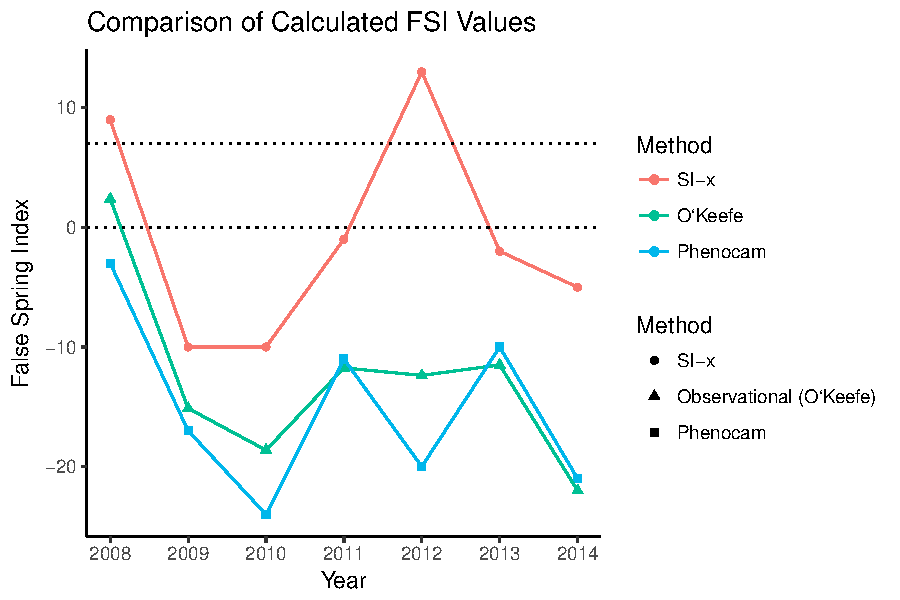
\includegraphics[width=\maxwidth]{figure/fsifig-1} 

}

\caption[False Spring Index (FSI) values from 2008 to 2014 vary across methodologies]{False Spring Index (FSI) values from 2008 to 2014 vary across methodologies. To calculate spring onset, we used the USA-NPN Extended Spring Index tool for the USA-NPN FSI values, which are in red (USA-NPN, 2016), long-term ground observational data for the observed FSI values, which are in green (O'Keefe, 2014), and near-surface remote-sensing canopy data for the PhenoCam FSI values, which are in blue (Richardson, 2015). The solid line at FSI=0 indicates a boundary between a likely false spring event or not, with positive numbers indicating a false spring likely occurred and negative numbers indicating a false spring most likely did not occur. The dotted line at FSI=7 indicates the 7 day threshold frequently used in false spring definitions, which suggests years with FSI values greater than 7 very likely had false spring events.}\label{fig:fsifig}
\end{figure}



\begin{figure}[H]

{\centering 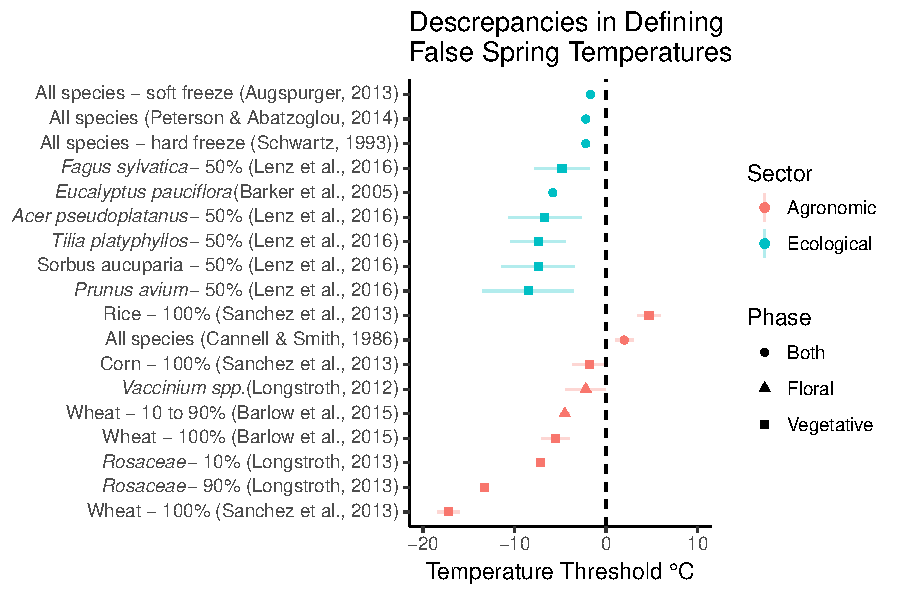
\includegraphics[width=\maxwidth]{figure/temp-1} 

}

\caption[A comparison of damaging spring freezing temperature thresholds across ecological and agronomic studies]{A comparison of damaging spring freezing temperature thresholds across ecological and agronomic studies. Each study is listed on the vertical axis along with the taxonomic group of focus. Next to the species name is the freezing definition used within that study (e.g. 100\% is 100\% lethality). Each point is the best estimate recorded for the temperature threshold with standard deviation if indicated in the study.}\label{fig:temp}
\end{figure}




\begin{figure}[H]

{\centering 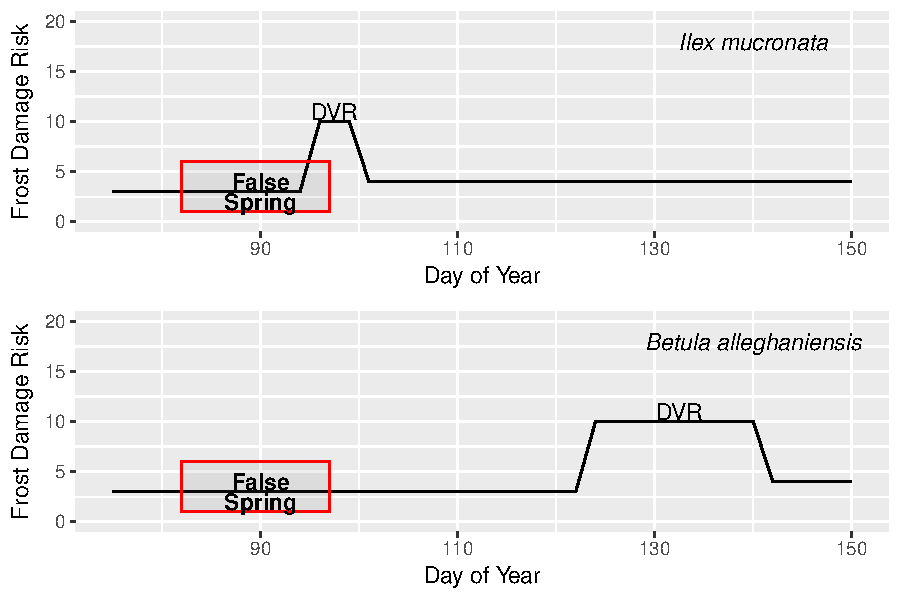
\includegraphics[width=\maxwidth]{figure/risk-1} 

}

\caption{Differences in spring phenology and false spring risk across two species: \textit{Ilex mucronata} (L.) and \textit{Betula alleghaniensis} (Marsh.). We mapped a hypothetical false spring event based on historical weather data and long-term observational phenological data collected at Harvard Forest (O'Keefe, 2014). In this scenario, \textit{Ilex mucronata}, which budbursts early and generally has a short period between budburst (light green squares) and leafout (dark green triangles), would be exposed to a false spring event during it's duration of vegetative risk (i.e. from budburst to leafout), whereas \textit{Betula alleghaniensis} would avoid it entirely (even though it has a longer duration of vegetative risk), due to later budburst.}\label{fig:risk}
\end{figure}



\begin{figure} [H] 
 \begin{center}
 %\textbf{How Major Cues of Spring Phenology Alter Vegetative Risk}\par\medskip
 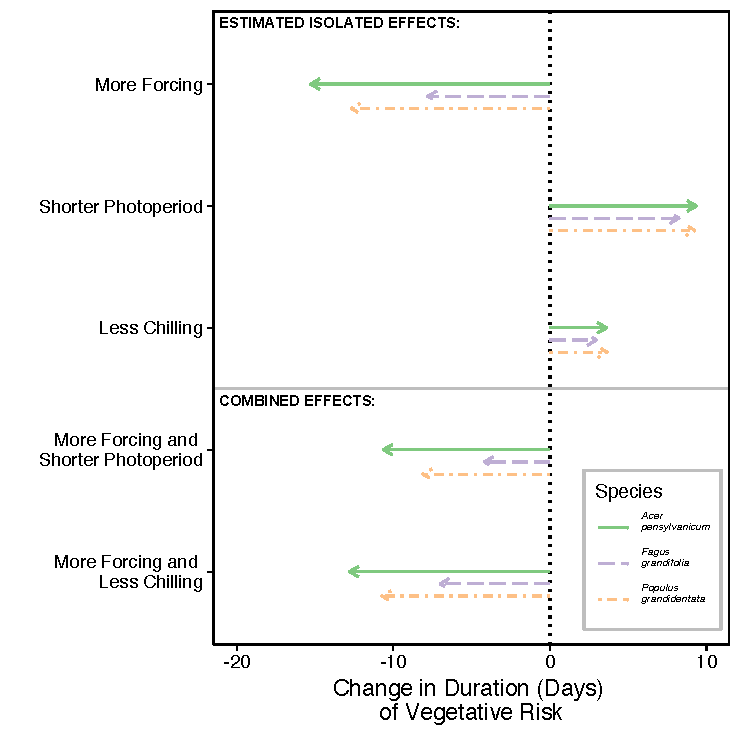
\includegraphics[width=12cm, height=12cm]{..//figure/Exp_plotTPS.pdf} 
 \caption{We examine the effects of phenological cues on the duration of vegetative risk across three species: \textit{Acer pensylvanicum}, \textit{Fagus grandifolia}, and \textit{Populus grandidentata}. `More Forcing' is a 5$^{\circ}$C increase in spring warming temperatures, `Shorter Photoperiod' is a 4 hour decrease in photoperiod and `Less Chilling' is a 30 day decrease in over-winter chilling. Along with the estimated isolated effects, we the show the combined predicted shifts in phenological cues with potential climate change effects on cues (i.e. more forcing with shorter photoperiod and more forcing with less chilling) and the subsequent shifts in duration of vegetative risk across species. To calculate the combined effects, we added the estimated isolated effects of each cue alone with the interaction effects for the relevant cues for each species. }\label{fig:dan} 
 \end{center}
 \end{figure}
% Need to say which treatments.

\begin{figure} [H] 
 \begin{center}
 %\textbf{Regional Differences in False Spring Risk}\par\medskip
 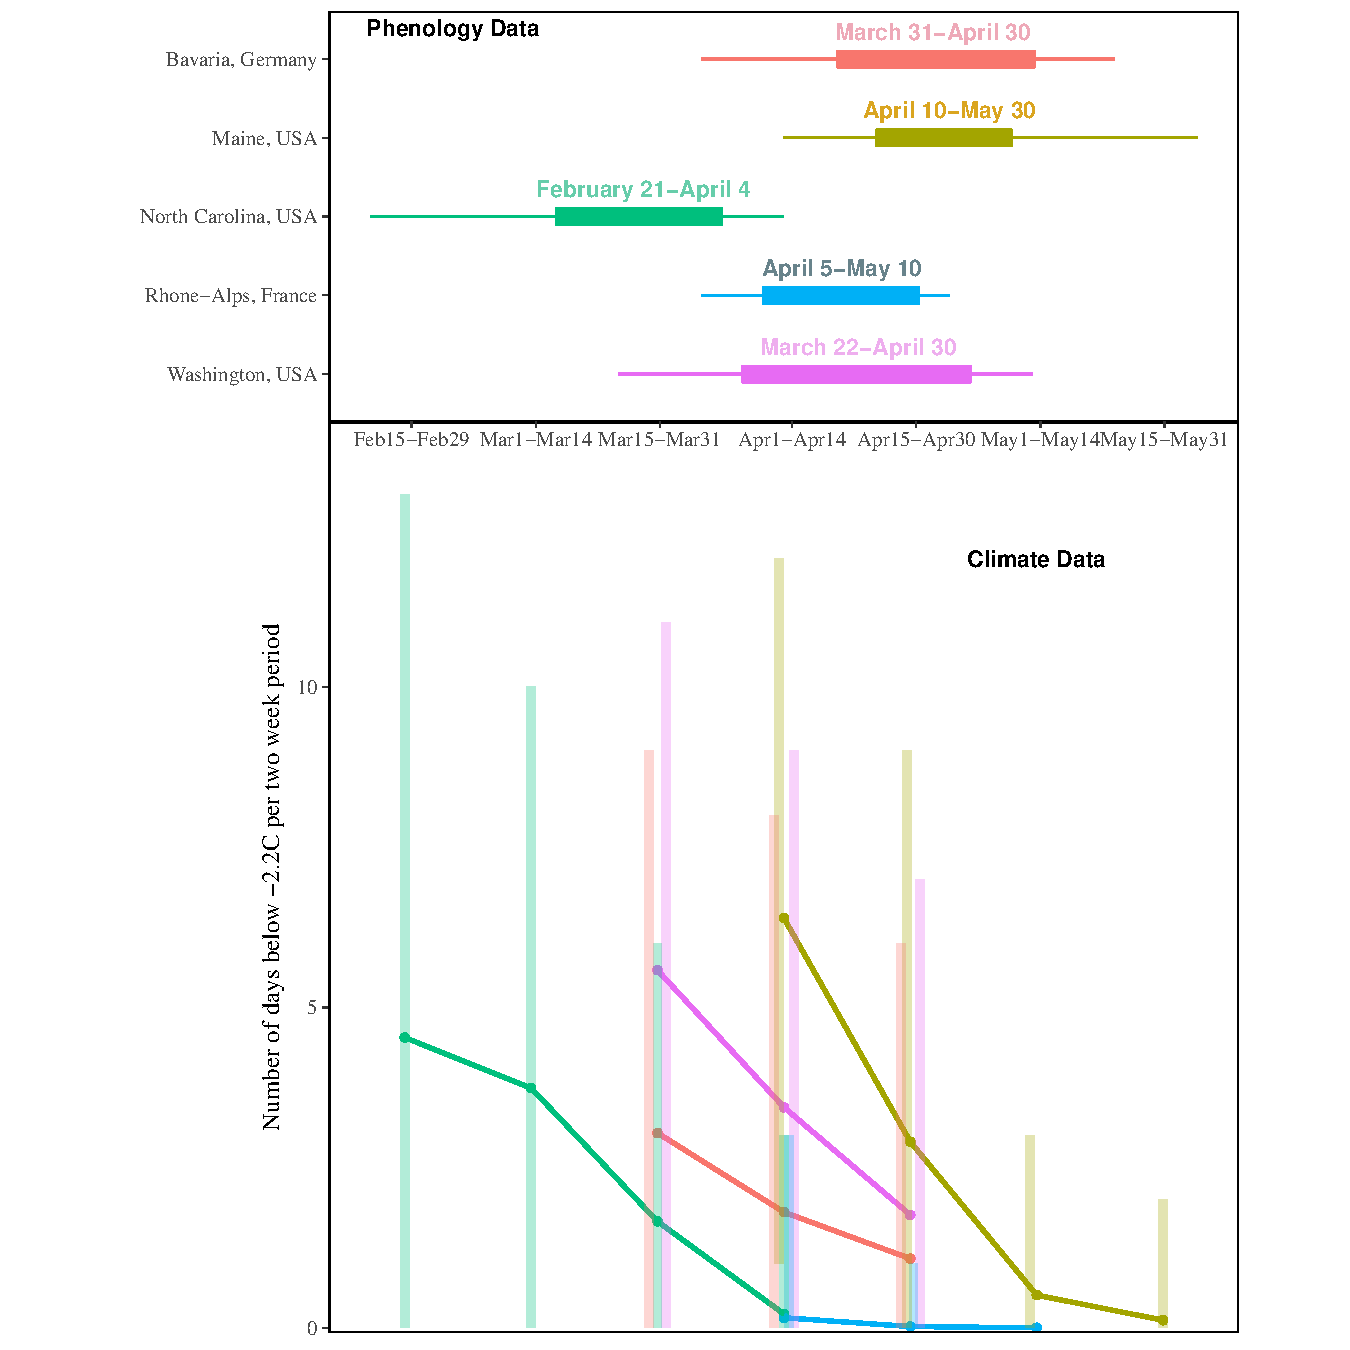
\includegraphics[width=16cm, height=18cm]{..//figure/RegRisk_flipped.pdf} 
 \caption{False spring risk can vary dramatically across regions. Here we show the period when plants are most at risk to tissue loss -- between budburst and leafout (upper, lines represent the range with the thicker line representing the interquartile range) and the variation in the number of freeze days (-2.2$^{\circ}$C) (Schwartz, 1993) that occurred on average over the past 50 years for five different sites (lower, bars represent the range, points represent the mean). Data come from USA-NPN SI-x tool (1981-2016) and observational studies (1950-2016) for phenology (Schaber \& Badeck, 2005; Soudani et al., 2012; USA-NPN, 2016; White et al., 2009) and NOAA Climate Data Online tool for climate (from 1950-2016). } \label{fig:region}  
 \end{center}
 \end{figure}

\end{document}
